% !TEX program = xelatex
% !BIB TS-program = biber

% **************************************************
% Document Class Definition
% **************************************************
\documentclass[%
    paper=A4,               % paper size --> A4 is default in Germany
    twoside=true,           % onesite or twoside printing
    openany,              % doublepage cleaning ends up right side
    parskip=full,           % spacing value / method for paragraphs
    chapterprefix=true,     % prefix for chapter marks
    11pt,                   % font size
    headings=normal,        % size of headings
    bibliography=totoc,     % include bib in toc
    listof=totoc,           % include listof entries in toc
    titlepage=on,           % own page for each title page
    captions=tableabove,    % display table captions above the float env
    draft=false,            % value for draft version
]{scrreprt}

\newcommand{\reportTitle}{\textcolor{ugent_blue}{Restricted Hartree Fock}} 
\newcommand{\reportName}{\textbf{Ruben Van der Stichelen}}
\newcommand{\reportSubject}{\emph{Programming project 3: the use of restricted Hartree Fock}}
\newcommand{\reportDate}{}
\newcommand{\reportVersion}{}

\usepackage[english]{babel} % babel system, adjust the language of the content
\PassOptionsToPackage{% setup clean thesis style
    figuresep=colon,%
    sansserif=true,%
    hangfigurecaption=false,%
    hangsection=true,%
    hangsubsection=true,%
    colorize=full,%
    colortheme=bluemagenta,%
    bibsys=biber,%
    bibfile=notes,%
    bibstyle=numeric-comp,%
    wrapfooter=false,%
}{cleanthesis}
\usepackage{cleanthesis}

\hypersetup{% setup the hyperref-package options
    pdftitle={\reportTitle},    %   - title (PDF meta)
    pdfsubject={\reportSubject},%   - subject (PDF meta)
    pdfauthor={\reportName},    %   - author (PDF meta)
    plainpages=false,           %   -
    colorlinks=false,           %   - colorize links?
    pdfborder={0 0 0},          %   -
    breaklinks=true,            %   - allow line break inside links
    bookmarksnumbered=true,     %
    bookmarksopen=true          %
}

\definecolor{ugent_blue}{RGB}{30, 100, 200}
\definecolor{sciences}{RGB}{45, 140, 168}

\usepackage{algorithm}              % http://ctan.org/pkg/algorithms
\usepackage{algpseudocode}          % http://ctan.org/pkg/algorithmicx
\usepackage{amsmath}
\usepackage{amsfonts}             % mathfrak
\usepackage{amssymb}              % \mathbb
\usepackage[mathscr]{euscript}    % \mathscr
\usepackage{chemmacros}
\usepackage{float}
\usepackage{graphicx}
\usepackage{interval}
\usepackage{mathtools}            % dcases, DeclareMathOperator, DeclairePairedDelimiter
\usepackage{physics}               % physics typesetting, especially bra-ket notation
\usepackage{siunitx}
\usepackage{subcaption}
\usepackage{tensor}
\usepackage{xcolor}
\usepackage{ifxetex}
\usepackage{multicol}
\usepackage{pdfpages}
\usepackage{epigraph}
\usepackage{bm}
\usepackage[normalem]{ulem}
\usepackage[version=3]{mhchem}
\usepackage[linewidth=1pt]{mdframed}
\usepackage{enumitem}
\usepackage{minted}


\DeclareSymbolFont{euleroperators}{U}{eur}{m}{n}
\SetSymbolFont{euleroperators}{bold}{U}{eur}{b}{n}

\makeatletter
\renewcommand{\operator@font}{\mathgroup\symeuleroperators}
\makeatother

% \usepackage[utf8]{inputenc} 


\ifxetex
  \usepackage{fontspec}
	% \setmainfont[
	% Path = ./,
	% BoldFont = UGentPannoText-SemiBold.otf,
	% ItalicFont = UGentPannoText-SemiLight.otf,
	% BoldItalicFont  = UGentPannoText-Medium.otf]
	% {UGentPannoText-Normal.otf}
	\newfontfamily\PannoSemiLight{UGentPannoText-SemiLight.otf}
	\newfontfamily\PannoMedium{UGentPannoText-Medium.otf}
	\newfontfamily\PannoSemiBold{UGentPannoText-SemiBold.otf}
	\newcommand{\PannoLarge}{\LARGE}
    \newcommand{\PannoNormalsize}{\large}
    \renewcommand{\helv}{\fontspec{UGentPannoText-Normal.otf}\fontsize{9}{11}\selectfont}
    \renewcommand{\book}{\fontspec{UGentPannoText-Normal.otf}\fontsize{11}{13}\selectfont}
    \renewcommand{\tgherosfont}{\fontspec{UGentPannoText-Normal.otf}}
    \renewcommand{\thesischapterfont}{\color{ctcolorblack}\huge\fontspec{UGentPannoText-Normal.otf}}
\else
  % \usepackage[utf8]{inputenc}           % Om niet ascii karakters rechtstreeks te kunnen typen
	\usepackage{lmodern}
	\usepackage[T1]{fontenc}
	\renewcommand{\familydefault}{\sfdefault}
	\newcommand{\PannoSemiLight}{}
	\newcommand{\PannoMedium}{}
	\newcommand{\PannoSemiBold}{}
	\newcommand{\PannoLarge}{\Large}
	\newcommand{\PannoNormalsize}{\normalsize}
\fi

\graphicspath{{img/}}
\linespread{1.2}
\numberwithin{equation}{section}
\renewcommand{\thesection}{\arabic{section}}

\title{\reportTitle}
\author{\reportName\\GQCG}

% **************************************************
% Document CONTENT
% **************************************************
\begin{document}

    \begin{titlepage}
        \hspace{-1cm}
\includegraphics[height=3cm]{faculty.png}
        \begin{center}
            \vspace{2cm}
            \Huge{\reportTitle} \\
            \vspace{1cm}
            \Large{\reportName} \\
            \vspace{2cm}
            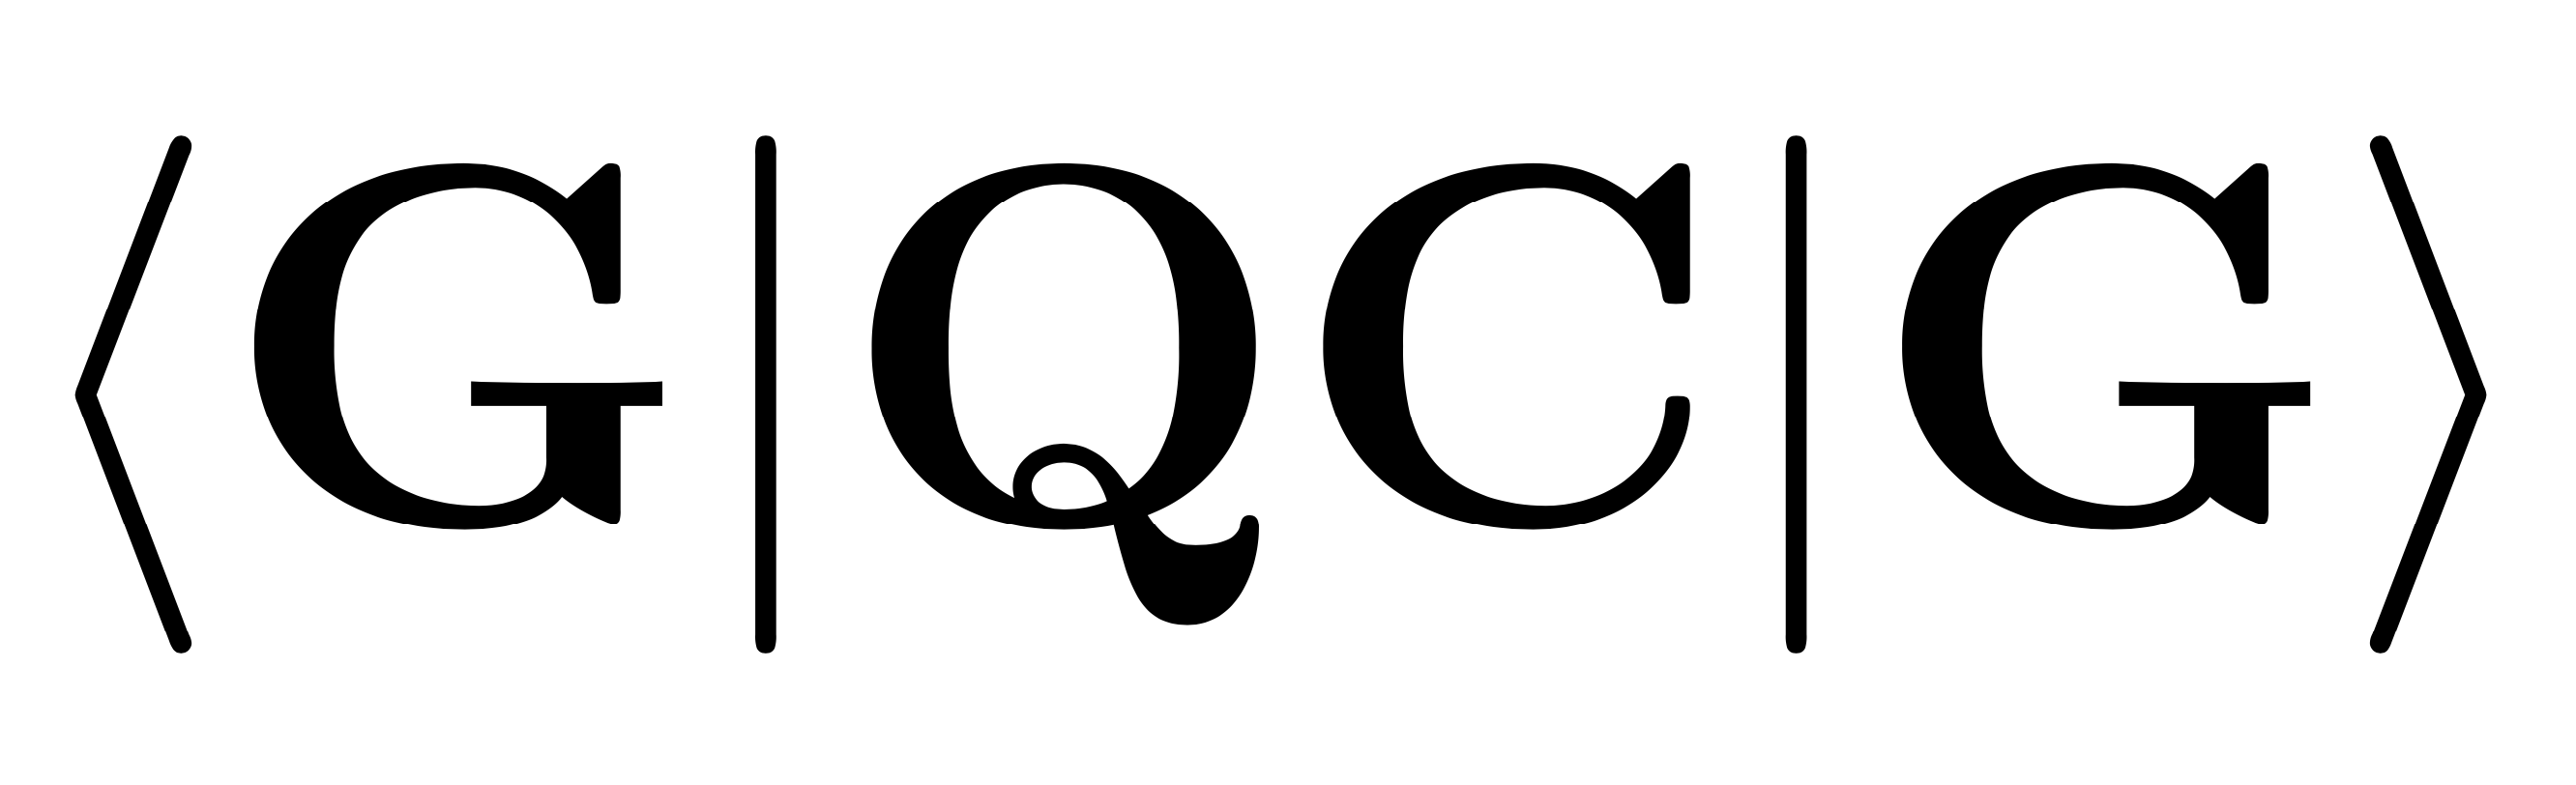
\includegraphics[height=2cm]{GQCG.png} \\
            \vspace{0.5cm}
            \large{Ghent University} \\ 
            \large{\today}
        \end{center}
        \vspace{4cm}
        \hspace{-1cm}
\includegraphics[height=4cm]{UGent.png}
    \end{titlepage}
    % --------------------------
    % rename document parts
    % --------------------------
    \renewcaptionname{english}{\figurename}{Fig.}
    \renewcaptionname{english}{\tablename}{Tab.}

    \setcounter{tocdepth}{2}		% define depth of toc

    % --------------------------
    % Body matter / main matter
    % --------------------------
    \pagenumbering{arabic}			% arabic page numbering
    \setcounter{page}{1}			% set page counter
    \pagestyle{maincontentstyle} 	% fancy header and footer

    % The following input statements correspond to the different chapters of these notes
    \section{Template section}

This is a report template. Citations can be used as via the included \emph{.bib} file \cite{acke2020}.
    \clearpage
    \section{Introduction}
    \label{sec:intro}
    This report will discuss the notebook we made on restricted Hartree-Fock theory. We will walk trough the notebook step by step and discuss what we see there. The same titles will be used, so you can follow along easily. Relevant parts of the code will be displayed.
    
    \section{Identifying the molecule}
    \label{sec:step1}
    In this first step we initiated the class molecule, which will be equipped with the necessary methods to do all the calculations we will be required to do. A molecule object has several properties that need to be defined first. 
    
    \begin{listing}[ht]
        \centering
        \inputminted[firstline=12, lastline=12, gobble=4]{python}{Hartree_FockL.py}
        \inputminted[firstline=23, lastline=36, gobble=4]{python}{Hartree_FockL.py}
        \caption{The parameters of the molecule object}
        \label{ls:Listing 1}
    \end{listing}
    In Listing \ref{ls:Listing 1} we the \mintinline{python}|__innit__| method of the molecule class. It sets us up with some of the information we will need later, namely the \mintinline{python}|psi4.core.Molecule| representation as \mintinline{python}|self.id|. We also see the wavefunction, basisset, integrals, occupied orbitals and a guess matrix. Since we will be doing Hartree-Fock calculations, which involve a lot of iterations, the molecule object will need a way to store the Fock matrix from the last iteration. From there we can then start for the next iteration. Hence the first method we actually have to define is a method that allows us to change this parameter.
    
    \begin{listing}[ht]
        \centering
        \inputminted[firstline=38, lastline=46, gobble=4]{python}{Hartree_FockL.py}
        \caption{The \mintinline{python}|setGuess| method}
        \label{ls: Listing 2}
    \end{listing}
    
    This is shown in Listing \ref{ls: Listing 2}. 
    
    \section{Prerequisite calculations}
    \label{sec:step2}
    
    In this section, we do some prerequisite calculations. These are relatively straightforward. In this step we added some methods to the class that allow us to calculate important properties like the nuclear repulsion kinetic energy and so on. The commands used are directly implemented from the psi4 package. They are listed in Table \ref{tab:my_label}
    
    \begin{table}[hp]
        \centering
        \begin{tabular}{c|c}
            command & property \\
            \hline
            \mintinline{python}|self.id.nuclear_repulsion_energy()| & nuclear repulsion energy \\
            \mintinline{python}|self.integrals.ao_overlap().np| & overlap matrix \\
            \mintinline{python}|self.integrals.ao_kinetic().np| & kinetic energy \\
            \mintinline{python}|self.integrals.ao_potential().np| & potential energy \\
            \mintinline{python}|self.displayE_kin() + self.displayE_pot()| & the core hamiltonian \\
            \mintinline{python}|self.integrals.ao_eri().np| & repulsion between electrons \\
        \end{tabular}
        \caption{Commands useed to calculate various properties}
        \label{tab:my_label}
    \end{table}
    We will not list the code for the various methods here, however when they appear in later blocks of code we will mention them.
    
    \section{The inital (guess) density matrix}
    \label{sec:step3}
    We will skip ahead to the function that gives us the density matrix and start from there.
    
    \begin{listing}[ht]
        \centering
        \inputminted[firstline=110, lastline=116, autogobble]{python}{Hartree_FockL.py}
        \caption{Getting the density matrix}
        \label{ls: Listing 3}
    \end{listing}
    
    This function uses the method \mintinline{python}|getEigenStuff|, which just calls the scipy function \mintinline{python}|linalg.eigh|. This solves the generelised eigenproblem posed by the Roothaan-Hall equation \eqref{eq:Roothaan-Hall}, for whatever matrix that is currently in the \mintinline{python}|self.guessMatrix| parameter.
    
    \begin{equation}\label{eq:Roothaan-Hall}
        \boldsymbol{FC} = \boldsymbol{SC}\epsilon
    \end{equation}
    
    C in Listing \ref{ls: Listing 3} then refers to \textbf{C} in Equation \eqref{eq:Roothaan-Hall}. The first matrix that we calculate the eigenvalues and eigenvectors from is the core Hamiltonian, so this will have to be stored as the \mintinline{python}|self.guessMatrix| before proceeding. Now we are set to build a Fock matrix.
    
    \section{Updating the Fock matrix}
    \label{sec:step4}
    
    \begin{listing}[ht]
        \centering
        \inputminted[firstline=119, lastline=124, autogobble]{pythonL}{.py}
        \caption{Getting the fock matrix}
        \label{ls: Listing 4}
    \end{listing}
     
     We see that the Fock-matrix uses some the density matrix and the electronic repulsion matrix and the Hamiltonian , which the molecule object call with the methods seen in Section \ref{sec:step2}. Since the density matrix depends on the current \mintinline{python}|self.guessMatrix|, the Fock matrix will also depend on it. We can then see that the new Fock matrix is always derived from the previous one, given that we update it during each step of the iteration.
     
     \section{The SCF energy}
     \label{sec:step5}
     From the Fock matrix we derived in the previous section, we can now calculate the electronic energy acoording to Equation \eqref{eq:energy}.
     
     \begin{equation} \label{eq:energy}
         E_{elek} = \frac{1}{2}\sum_{\mu\nu}D_{\mu\nu}*(H_{\mu\nu} + F_{\mu\nu})
     \end{equation}
     In python this looks like Lising \ref{ls: Listing 5}.
     
     \begin{listing}[ht]
         \centering
        \inputminted[firstline=127, lastline=132, autogobble]{python}{Hartree_FockL.py}
        \caption{Calculating the energy}
        \label{ls: Listing 5}
     \end{listing}
     The total energy is merely the sum of this electronic energy and the nuclear repulsion energy. We have a method for that defined in Section \ref{sec:step2}.
     
     \section{Test for convergence}
     \label{sec:step6}
    Now we only need to bring this all together to get the final energy. This is done in the function \mintinline{python}|iterator| as seen in Listing \ref{ls: Listing 6}.
    
     \begin{listing}[H]
         \centering
        \inputminted[firstline=142, lastline=178, autogobble]{python}{Hartree_FockL.py}
        \caption{the iteration}
        \label{ls: Listing 6}
     \end{listing}
     First we need to set up the parameters before we start iterating. That is done in the first block of code. Then we start a while loop, that will stop iterating once we have reached convergence, or when we have reached the maximum amount of iterations. Inside the loop, we see four blocks of code. The calculating block provides us with the energy of the molecule for the given \mintinline{python}|self.guessMatrix|. The next block will generate new matrices for the next iterative step. In the comparing block we check the conditions for convergence. For this we need four values, the old and new energies and the old and new distance matrices. For more information, see Subsection \ref{subsec:step6.1}. For now we will continue to walk trough the code. After the comparing block we move to the final block, which sets us up for the next iteration. This iterations energy is stored, as well as the density matrix. We print out a line that summarises all the relevant values for this iteration. We can then move on to the next iterative step until the while loop finds one of its conditions is no longer met.
     
     \subsection{on comparing values}
     \label{subsec:step6.1}
     In Listing \ref{ls: Listing 6} we can see that the energy has a much more severe criterion than the density matrix. The reason here has to do with the way these differences are calculated. Given that the energy is calculated using a product of the density matrix with itself. (or something that looks like a product) Indeed we see in Equation \ref{eq:energy} that the energy is calculated using a product of the Fock matrix with the density matrix, when this Fock matrix is already contains the density matrix as can be seen in Equation \ref{eq: fock matrix}. 
     
     \begin{equation} \label{eq: fock matrix}
         \boldsymbol{F}_{\mu\nu} = \boldsymbol{H}_{\mu\nu} + \sum^{AO}_{\lambda\sigma}[(\mu\nu|\lambda\sigma) - \frac{1}{2}(\mu\lambda|\nu\sigma)]
     \end{equation}
     For this reason the error on the energy will always be bigger than the error on the density matrix, so we have to define the energy convergence somewhat stricter. If you would define the convergence criterion of the energy using the same value for the density, you will notice that the density criterion will never be reached. If we define the criteria correctly we would also notice that we do not need to enforce both of them. We will later see that when one condition applies, the other is automatically fulfilled as well. It would have sufficed to enforce only the energy criterion for example.
     
     \section{Some examples}
     \label{sec: examples}
     In this section, we will display some of the results from our calculations for two example systems, water and methane. We will give a display of the output as generated by the functions we discussed above.
     
     \subsection{water}
     \label{subsec:water}
    
    \begin{minted}{python}[ht]
    0, E_tot: -73.28579642, E_elek: -81.28816348, deltaE: -81.2881634, rmsD:  14.05298222
    1, E_tot: -74.82812538, E_elek: -82.83049244, deltaE: -1.54232896, rmsD:  3.17285816 
    2, E_tot: -74.93548800, E_elek: -82.93785506, deltaE: -0.10736262, rmsD:  0.65858574 
    3, E_tot: -74.94147774, E_elek: -82.94384480, deltaE: -0.00598974, rmsD:  0.24093051 
    4, E_tot: -74.94197200, E_elek: -82.94433906, deltaE: -0.00049425, rmsD:  0.08612099
    5, E_tot: -74.94205606, E_elek: -82.94442312, deltaE: -0.00008407, rmsD:  0.04061885
    6, E_tot: -74.94207442, E_elek: -82.94444148, deltaE: -0.00001836, rmsD:  0.01827516
    7, E_tot: -74.94207865, E_elek: -82.94444571, deltaE: -0.00000423, rmsD:  0.00892060
    8, E_tot: -74.94207963, E_elek: -82.94444669, deltaE: -0.00000098, rmsD:  0.00425406
    9, E_tot: -74.94207986, E_elek: -82.94444692, deltaE: -0.00000023, rmsD:  0.00205358
    10, E_tot: -74.94207991, E_elek: -82.94444697, deltaE: -0.00000005, rmsD:  0.00098889
    11, E_tot: -74.94207992, E_elek: -82.94444699, deltaE: -0.00000001, rmsD:  0.00047710
    12, E_tot: -74.94207993, E_elek: -82.94444699, deltaE: -0.00000000, rmsD:  0.00023011
    13, E_tot: -74.94207993, E_elek: -82.94444699, deltaE: -0.00000000, rmsD:  0.00011102
    14, E_tot: -74.94207993, E_elek: -82.94444699, deltaE: -0.00000000, rmsD:  0.00005356
    \end{minted}
    Here we see the the amount of iterations before the convergence is reached and all parameters calculated during that iteration. Furtermore we can use the \mintinline{python}|oeprop| method to get the dipole and nuclear charges.
    \begin{table}[ht]
        \centering
        \begin{tabular}{c|c}
             total dipole moment & 0.6034  \\
             \hline
             nuclear charges &  \\ 
             \hline
             O & -0.25302 \\
             H & 0.12651 \\
             H & 0.12651 \\
        \end{tabular}
        \caption{Some properties of water}
        \label{tab:number2}
    \end{table}
     
    \subsection{methane}
    \label{subsec:methane}
     
     \begin{minted}{python}
    0, E_tot: -36.08344857, E_elek: -49.58075304, deltaE: -49.58075304, rmsD:  35.9980315
    1, E_tot: -39.56451342, E_elek: -53.06181788, deltaE: -3.48106485, rmsD:  4.73662689
    2, E_tot: -39.72183632, E_elek: -53.21914079, deltaE: -0.15732290, rmsD:  0.79654919
    3, E_tot: -39.72669300, E_elek: -53.22399746, deltaE: -0.00485667, rmsD:  0.14041648
    4, E_tot: -39.72684535, E_elek: -53.22414982, deltaE: -0.00015236, rmsD:  0.02394664
    5, E_tot: -39.72685016, E_elek: -53.22415462, deltaE: -0.00000480, rmsD:  0.00443984
    6, E_tot: -39.72685031, E_elek: -53.22415477, deltaE: -0.00000015, rmsD:  0.00072904
    7, E_tot: -39.72685032, E_elek: -53.22415478, deltaE: -0.00000001, rmsD:  0.00014205
    8, E_tot: -39.72685032, E_elek: -53.22415478, deltaE: -0.00000000, rmsD:  0.00002652
    \end{minted}
     
     \begin{table}[ht]
        \centering
        \begin{tabular}{c|c}
             total dipole moment & 0.0000  \\
             \hline
             nuclear charges &  \\ 
             \hline
             C & -0.26031 \\
             H & 0.06508 \\
             H & 0.06508 \\
             H & 0.06508\\
             H & 0.06508 \\
        \end{tabular}
        \caption{Some properties of methane}
        \label{tab:number3}
    \end{table}
    % **************************************************
    % End of Document CONTENT
    % **************************************************
    \end{document}
